%!TEX root = main.tex
\documentclass[main.tex]{subfiles}

\begin{document}

\section{Conclusion}

One of the primary aims of this project was to implement some kind of physical system to sit between a landline and an analogue phone, and intercept calls. This was clearly performed. In determining the legitimacy of incoming calls, the system was successful within limits. Voice prompts and messages prevent robot calls from coming through, but also frustrate and annoy legitimate callers. Audio content analysis to extract speech, and have it analysed for keywords worked correctly, but were limited by the static lists and dynamic nature of scammers. However, it is markedly different of existing commercially available products as it does not require Caller ID. While there are still a wide variety of other methods that can be employed, the system that was made in this project does present a base on which to continue the conflict between scammers and vulnerable users around the world (Figure \ref{fig:memes}).

\begin{figure}[htb]
	\captionsetup[subfigure]{position=b}
        \centering
        \begin{subfigure}{0.4\textwidth}
                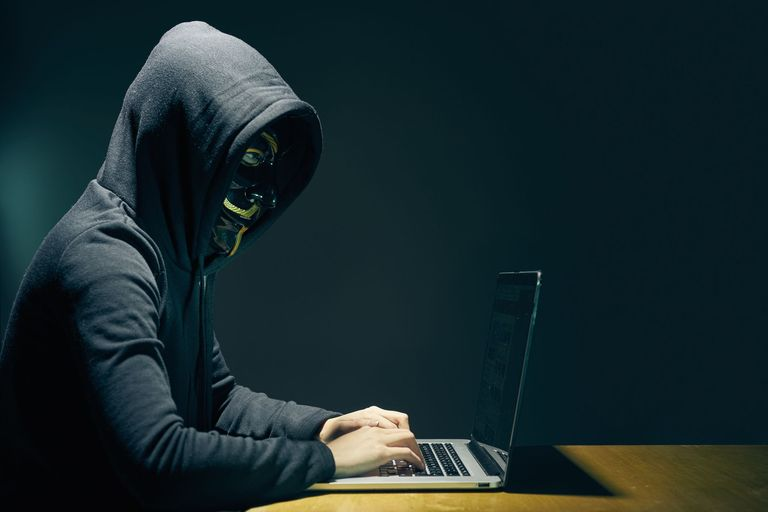
\includegraphics[width=\textwidth]{pics/hacker}
                \caption{Malicious scammers \cite{hacker}.}
                \label{fig:hacker}
        \end{subfigure}
        ~
		\begin{subfigure}{0.4\textwidth}
                
\includegraphics[width=\textwidth]{pics/harold}
                \caption{Unsuspecting innocents \cite{harold}.}
                \label{fig:harold}
        \end{subfigure}
	\caption{The standoff between malicious scammers and unsuspecting innocents.}
	\label{fig:memes}
\end{figure}
\vspace{-0.75cm}
\section{Future Work}
With more time, additional data can be collected for testing different methods, particular those involving audio transcription and Caller ID. With more data, there is a better change of locating keywords or notable patterns. Interaction with telephone companies could also be considered. With their direct connection to the infrastructure and industry, it would be interesting to note how (if any) scam prevention is done on a wide scale and how this relates to all the academic work encountered.
\\\\
While the idea of a physical circuit board to interface with the line on a lower level was dropped early on, it could be interesting, both as a learning experience, and as an option that might open more identification methods. As for the system itself, a nicer packaging for the various components or a size reduction could make it a nice hobby kit. And with the open-source nature of all the software used, allowing a larger community to work on it give many more possibilities.

\end{document}
